\documentclass{article}
\usepackage[utf8]{inputenc}
\usepackage{textcomp}
\usepackage{graphicx}
\usepackage{float}
\usepackage{array}
\usepackage{amsmath} % Math aligning equation
\usepackage{verbatim} % Command \verb
\usepackage{titlesec} % Righe di separazione


% Tabelle
\usepackage{tabu}
\usepackage{caption} 
\captionsetup[table]{skip=2pt}

% Impostazioni di pagina e margini
\usepackage[a4paper, margin=2.54cm]{geometry}

% Spacing nelle liste
\usepackage{enumitem}
\setlist{topsep=2pt, itemsep=2pt, partopsep=2pt, parsep=2pt}

% Cambio di nome di contenuti Latex
\renewcommand*\contentsname{Indice}
\renewcommand{\figurename}{Figura}
\renewcommand{\tablename}{Tabella}

% Checkmarks
\usepackage{pifont}
\newcommand{\cmark}{\ding{51}} % V
\newcommand{\xmark}{\ding{55}} % X

% Header & Footer
\usepackage{fancyhdr}
\pagestyle{fancy}
\fancyhf{}
\lhead{Progetto finale di Reti Logiche - a.a. 2018/2019}
\rhead{Motta Dennis}
\cfoot{\thepage}

% Titolo e informazioni
\title{Progetto finale di Reti Logiche}
\author{Motta Dennis - Matricola n. 865833}
\date{Anno Accademico 2018/2019}


\begin{document}

\maketitle
\tableofcontents


%%%%%%%%%%%%%%%%%%%%%%%%%%%%%%%%%%%%%%%%%%%%
%%%%%%%%%%%%%%% INTRODUZIONE %%%%%%%%%%%%%%%
%%%%%%%%%%%%%%%%%%%%%%%%%%%%%%%%%%%%%%%%%%%%
\pagebreak
\section{Introduzione} \label{subsection-introduz}
Il mio obiettivo per questo progetto, oltre a creare un design funzionante in pre e post sintesi che rispetti le specifiche, è stato quello di creare un componente che arrivasse al risultato il più velocemente possibile, sfruttando quindi ogni ciclo di clock, ma senza dimenticare di scrivere codice semplice, senza ripetizioni e di facile manutenzione.\\
Queste scelte progettuali portano anche alcuni svantaggi: con un focus sulla velocità totale le caratteristiche di massima frequenza del clock e di area occupata passano in secondo piano. Non si è scelto un focus sull'area occupata in quanto la FPGA scelta ha centinaia di migliaia di Flip-Flop e LUT. Anche un focus su una maggiore frequenza di clock è stato messo in secondo piano in quanto il progetto ha già un periodo di clock di 100 ns dato da specifica.

\subsection{Funzionamento in sintesi}
In una breve sintesi introduttiva, si può rappresentare il funzionamento di base e non ottimizzato del componente attraverso un numero finito di step (e ciò verrà rappresentato architetturalmente attraverso una macchina a stati finiti):
\begin{enumerate}
    \item Reset e attesa del segnale di start.
    \item Inizializzazione degli output del componente mandando la richiesta di lettura della maschera d'ingresso alla RAM.
    \item Lettura e salvataggio in un registro della maschera di ingresso.
    \item Lettura e salvataggio della X del punto da valutare.
    \item Lettura e salvataggio della Y del punto da valutare.
    \item Lettura e salvataggio della X del 1° centroide.
    \item Lettura della Y del 1° centroide. Se il centroide va considerato per la maschera d'ingresso si calcola la distanza tra il punto da valutare e il centroide. Se questa distanza è minore della distanza minima la si salva e si sovrascrive la maschera di uscita temporanea, se essa invece è uguale alla distanza minima si pone il primo bit a '1' nella maschera di uscita temporanea.
    \item In modo equivalente 2°, 3°, 4°, 5°, 6° e 7° centroide... \addtocounter{enumi}{11}
    \item Lettura e salvataggio della X del 8° centroide.
    \item Lettura della Y del 8° centroide. Se il centroide va considerato per la maschera d'ingresso si calcola la distanza tra il punto da valutare e il centroide. Se questa distanza è minore della distanza minima la si salva e si sovrascrive la maschera di uscita temporanea, se essa invece è uguale alla distanza minima si pone l'ottavo bit a '1' nella maschera di uscita temporanea.\\
    Infine, avendo raggiunto l'ultimo centroide si scrive sulla RAM la maschera di uscita trovata.
    \item Segnalazione di fine elaborazione usando il segnale \verb^o_done^; Attesa del segnale di fine (\verb^i_start^ posto a '0') che ci permetterà di ritornare allo step 1 per una possibile successiva elaborazione.
\end{enumerate}

\subsection{Obiettivo velocità} \label{subsection-ob-vel}
Per raggiungere l'obiettivo della velocità si è dovuto tenere in considerazione le limitazione della RAM: a ogni ciclo di clock solo una lettura o una scrittura. La RAM quindi ha imposto un limite massimo di velocità raggiungibile. Per raggiungere questo limite si è creato un codice in cui l'elaborazione e la presentazione dei segnali di output avvenisse nello stesso ciclo di clock in cui viene fatta la lettura del dato.\\
Una volta raggiunto il limite imposto dalla RAM si sono applicate alcune ottimizzazioni per raggiungere la massima velocità nel calcolo della maschera di uscita:
\begin{enumerate}
    \item Si evita la lettura sia del valore X che del valore Y di centroidi che sono disattivati nella maschera di ingresso
    \item Viene presentato il risultato immediatamente quando i bit attivati (bit '1') nella maschera di ingresso sono in numero uguale a 0 o 1 (esempio: "00100000"). In questi casi la maschera di output è necessariamente identica alla maschera di ingresso.
    \item Si passa al centroide successivo (tenendo in considerazione l'ottimizzazione n.1) quando alla lettura del valore X del centroide si trova che la distanza sulle ascisse del centroide col punto da valutare è maggiore della distanza minima fino a quel momento trovata. (esempio: distanza minima = 4; punto da valutare X = 12; centroide X = 78; in questo caso la distanza sulle ascisse è pari a \(78-12=66\) che è già maggiore della distanza minima, si passa quindi al centroide successivo)
\end{enumerate}

\subsection{Obiettivo codice semplice}
Per scrivere codice semplice e di facile manutenzione si è deciso di usare il meno possibile funzionalità algoritmiche (process), ciò per cercare di non utilizzare il linguaggio VHDL come se fosse un linguaggio di programmazione software. Il codice è quindi organizzato in diverse funzionalità, tutte inserite in un singolo modulo (entity); questa decisione puramente personale è stata presa per non complicare un codice in sostanza semplice.\\
Infine si sono create due costanti e un generic per rendere il codice facilmente espandibile a possibili modifiche:
\begin{itemize}
    \item \verb^MEM_BITS^ : costante che indica il numero di bit per un indirizzo di memoria. Per soddisfare la specifica di default è assegnato il valore 16.
    \item \verb^CELL_BITS^ : costante che indica il numero di bit in una cella di memoria che si assume equivalente al numero di centroidi da analizzare. Per soddisfare la specifica di default è assegnato il valore 8.
    \item \verb^START_ADDRESS^ : generic che facilita la modifica dell'indirizzo iniziale di memoria (dove è quindi salvata la maschera d'ingresso). Per soddisfare la specifica di default è assegnato il valore 0.
\end{itemize}

\subsection{Note aggiuntive sulla specifica}
Si è assunto che il componente deve essere in grado di eseguire elaborazioni una successiva all'altra anche in assenza di un segnale di reset.

\vspace{4mm}
\titlerule[0.4pt]


%%%%%%%%%%%%%%%%%%%%%%%%%%%%%%%%%%%%%%%%%%%%
%%%%%%%%%%%%%%% ARCHITETTURA %%%%%%%%%%%%%%%
%%%%%%%%%%%%%%%%%%%%%%%%%%%%%%%%%%%%%%%%%%%%
\pagebreak
\section{Architettura}

\subsection{Macchina a Stati Finiti}
Il funzionamento alla base del componente è stato implementato attraverso una FSM che usa come segnale di ingresso \verb^i_start^. In realtà, il passaggio agli stati successivi è dato da condizioni più complesse che permettono l'ottimizzazione, ciò verrà approfondito poco più avanti nella sezione \ref{subsection-ottimiz-fsm}.
La FSM non ottimizzata è rappresentata in figura \ref{fig:FSM}, mentre ciò che ogni stato rappresenta è spiegato più in dettaglio in tabella \ref{tab:FSM}.

\begin{figure}[H]
    \centering
    \caption{Macchina a Stati Finiti implementata}
    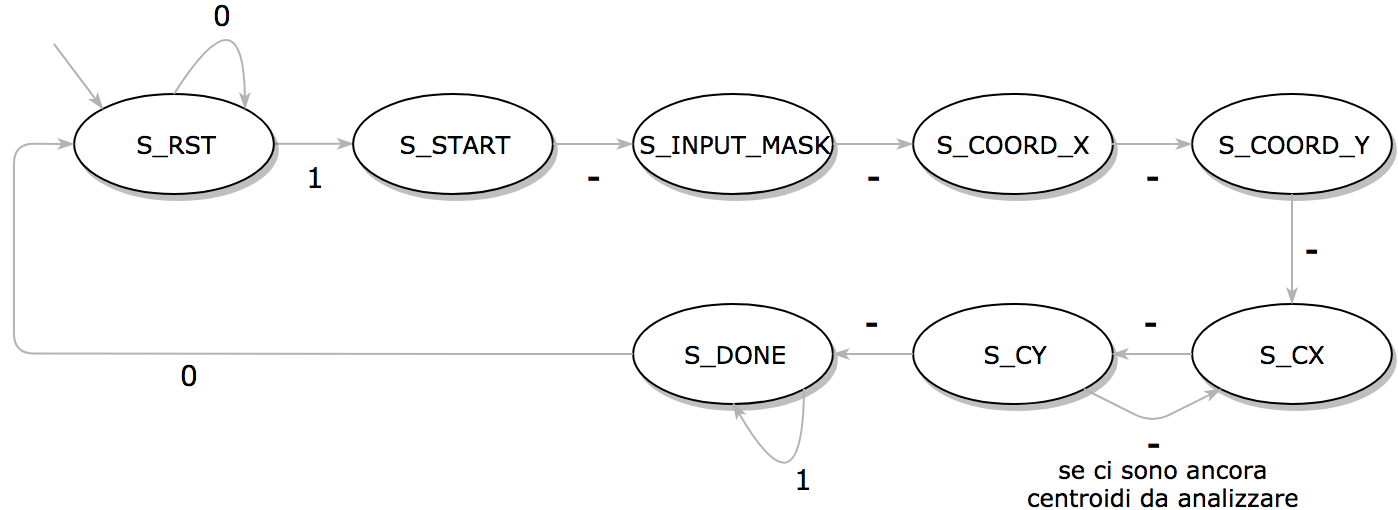
\includegraphics[width=1.0\textwidth]{images/FSM.png}
    \label{fig:FSM}
\end{figure}

\setlength\intextsep{0mm}
\begin{table}[H]
    \centering
    \caption{Stati della FSM}
    \begin{tabu*} to 1.0\textwidth { | X[1] | X[4.0] | }
        \hline
        \verb^S_RST^ & Stato di partenza della FSM e stato in cui si andrà in presenza di un segnale \verb^i_rst^. Alla ricezione di un segnale \verb^i_start^ si passa allo stato \verb^S_START^.\\
        \hline
        \verb^S_START^ & Stato iniziale. In questo stato viene fornito alla RAM l'indirizzo della maschera di ingresso specificato dal generic \verb^START_ADDRESS^. \\
        \hline
        \verb^S_INPUT_MASK^ & Stato in cui il componente legge e salva in un registro la maschera di ingresso che gli è arrivata da memoria. \\
        \hline
        \verb^S_COORD_X^ & Stato in cui il componente legge e salva in un registro la X del punto da valutare che gli è arrivata da memoria. \\
        \hline
        \verb^S_COORD_Y^ & Stato in cui il componente legge e salva in un registro la Y del punto da valutare che gli è arrivata da memoria. \\
        \hline
        \verb^S_CX^ & Lettura e salvataggio delle X dei centroidi. \\
        \hline
        \verb^S_CY^ & Lettura delle Y dei centroidi. Si calcola la distanza tra il punto da valutare e il centroide, se essa è minore della distanza minima si salva questa nuova distanza e si sovrascrive la maschera di uscita temporanea, se essa invece è uguale alla distanza minima si pone il bit corrispondente a '1' nella maschera di uscita temporanea. Infine, se il centroide corrente è l'ultimo si scrive la maschera di uscita sulla RAM. \rule[-1.0ex]{0pt}{1.0ex} \\
        \hline
        \verb^S_DONE^ & Stato in cui si segnala che il risultato è stato scritto in RAM: \verb^o_done^ è portato ad '1'. Alla ricezione di \verb^i_start^ uguale a '0' si riporta la macchina in \verb^S_RST^ per una possibile successiva elaborazione. \\
        \hline
    \end{tabu*}
    \label{tab:FSM}
\end{table}

\subsubsection{Ottimizzazioni effettuate} \label{subsection-ottimiz-fsm}
Per arrivare al risultato nel modo più veloce possibile si sono applicate alcune ottimizzazioni già introdotte nella sezione \ref{subsection-ob-vel} a pagina \pageref{subsection-ob-vel}. Vediamo più in dettaglio gli effetti sulla FSM:
\begin{enumerate}
    \item Si evita la lettura di centroidi che sono disattivati nella maschera di ingresso, ciò significa che lo stato \verb^S_CX^ verrà percorso un numero di volte pari al numero di bit attivi nella maschera di ingresso. 
    \item Alla lettura della maschera di ingresso che avviene nello stato \verb^S_INPUT_MASK^, se si scopre che essa ha 0 o 1 bit attivati, si passa direttamente allo stato \verb^S_DONE^ scrivendo il risultato nella RAM.
    \item Alla lettura della X di un qualsiasi centroide che avviene nello stato \verb^S_CX^, se si trova che la distanza sulle ascisse tra il centroide e il punto da valutare è maggiore della distanza minima fino a quel momento trovata, si passa al centroide successivo rimanendo quindi nello stato \verb^S_CX^ (il centroide successivo è calcolato tenendo presente l'ottimizzazione n.1).
\end{enumerate}

\subsection{Schema funzionale} \label{subsection-schema-funz}
\begin{figure}[H]
    \centering
    \caption{Schema funzionale del componente}
    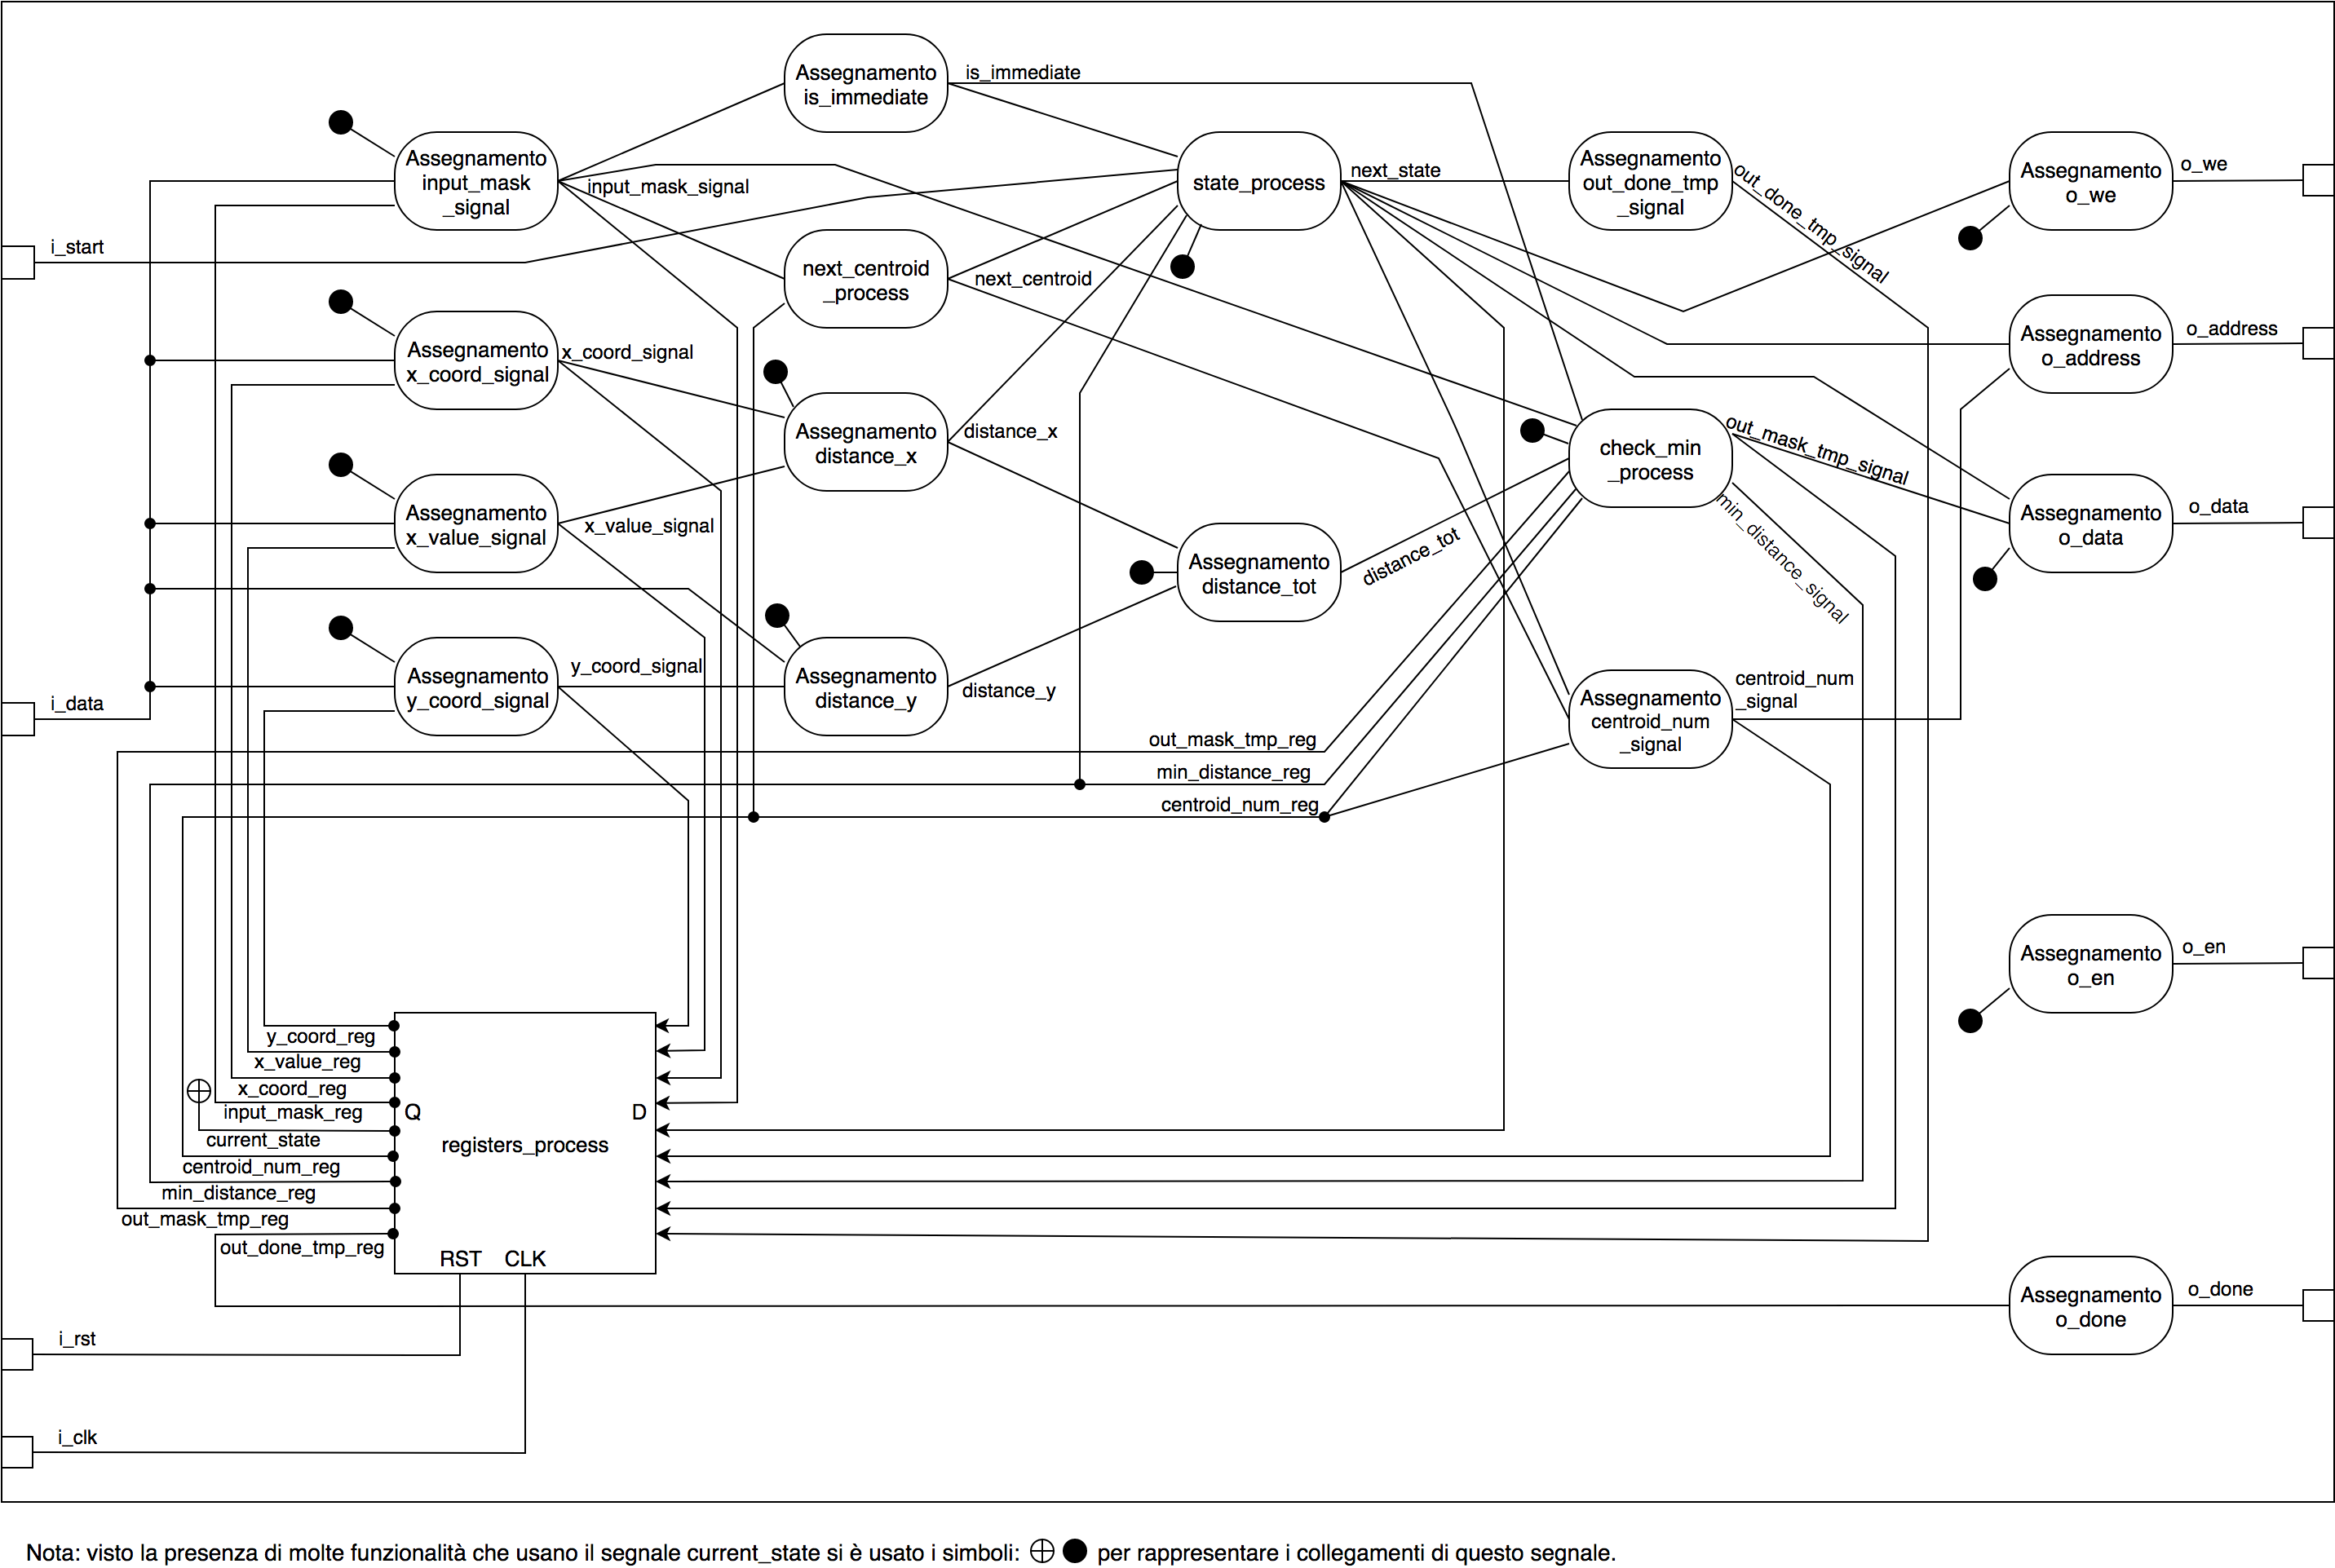
\includegraphics[width=1.0\textwidth]{images/Schema.png}
    \label{fig:Schema}
\end{figure}

\subsubsection{Registri}
Come si può vedere dallo schema funzionale, \verb^registers_process^ permette di creare 9 registri con lo scopo di salvare il valore di alcuni importanti segnali:
\begin{itemize}
    \item \verb^current_state^ : stato corrente della FSM.
    \item \verb^centroid_num_reg^ : centroide corrente.
    \item \verb^input_mask_reg^ : maschera d'ingresso.
    \item \verb^x_coord_reg^ : X del punto da valutare.
    \item \verb^y_coord_reg^ : Y del punto da valutare.
    \item \verb^x_value_reg^ : X del centroide corrente.
    \item \verb^min_distance_reg^ : distanza minima trovata.
    \item \verb^out_mask_tmp_reg^ : maschera d'uscita temporanea.
    \item \verb^out_done_tmp_reg^ : valore da dare a \verb^o_done^ al prossimo ciclo di clock, si è usato un registro per evitare alee statiche sul segnale che avrebbero compromesso il funzionamento.
\end{itemize}
N.B.: Si è usata la convenzione che i segnali \verb^*_signal^ rappresentano l'ingresso dei registri mentre i segnali \verb^*_reg^ le uscite (eccetto per il registro dello stato della FSM che usa \verb^current_state^ e \verb^next_state^).

\subsubsection{Funzionalità in dettaglio}
Vediamo ora più in dettaglio lo scopo di ogni funzionalità:
\begin{itemize}
    \item Assegnamento \verb^x_coord_signal^, assegnamento \verb^x_value_signal^, assegnamento \verb^y_coord_signal^, assegnamento \verb^input_mask_signal^: assegna all'ingresso del relativo registro il giusto segnale, che può essere il segnale \verb^i_data^ oppure il valore di uscita del registro.
    \item Assegnamento \verb^is_immediate^ : segnala se la maschera di ingresso permette di avere una risposta immediata (cioè se ha 1 oppure 0 bit attivati). Per arrivare al risultato si è utilizzato un famoso "trucchetto": avere un bit attivato significa essere una potenza di 2. Ed N è una potenza di 2 se \(N \& (N-1)\) = 0. Dove \& rappresenta l'and bit a bit. Questa funzionalità permette la realizzazione dell'ottimizzazione n.2 della sezione \ref{subsection-ottimiz-fsm} a pagina \pageref{subsection-ottimiz-fsm}.
    \item \verb^next_centroid_process^ : trova il valore del possibile prossimo centroide utilizzando il valore del centroide corrente e la maschera d'ingresso, salta quindi i centroidi non da considerare. Questa funzionalità permette la realizzazione dell'ottimizzazione n.1 della sezione \ref{subsection-ottimiz-fsm} a pagina \pageref{subsection-ottimiz-fsm}.
    \item Assegnamento \verb^distance_x^ : calcola la distanza sulle ascisse.
    \item Assegnamento \verb^distance_y^ : calcola la distanza sulle ordinate.
    \begin{sloppypar}\item Assegnamento \verb^distance_tot^ : calcola la distanza totale, cioè la somma di \verb^distance_x^ e \verb^distance_y^.\end{sloppypar}
    \item \verb^state_process^ : gestisce lo stato della FSM. I segnali in ingresso \verb^current_state^ e \verb^i_start^ servono alla FSM di base mentre gli altri segnali permettono le ottimizzazioni specificate nella sezione \ref{subsection-ottimiz-fsm} a pagina \pageref{subsection-ottimiz-fsm}. Il segnale \verb^next_centroid^ permette l'ottimizzazione n.1. Il segnale \verb^is_immediate^ permette l'ottimizzazione n.2. I segnali \verb^distance_x^ e \verb^min_distance_reg^ permettono l'ottimizzazione n.3.
    \item Assegnamento \verb^out_done_tmp_signal^ : assegna all'ingresso del registro il valore da dare a \verb^o_done^ al prossimo ciclo di clock. Il segnale è portato a '1' quando il prossimo stato specificato in \verb^next_state^ è \verb^S_DONE^.
    \item \verb^check_min_process^ : controlla se il centroide corrente è a distanza minima usando \verb^distance_tot^. Se questa distanza è minore della distanza minima la si assegna a \verb^min_distance_signal^ e si sovrascrive \verb^out_mask_tmp_signal^, se essa invece è uguale alla distanza minima si attiva il bit corrispondente al centroide in \verb^out_mask_tmp_signal^.
    \item Assegnamento \verb^centroid_num_signal^ : trova il valore effettivo di quello che sarà il prossimo centroide. Il centroide successivo dipende da \verb^next_state^, cioè lo stato in cui andrà la FSM: se il prossimo stato è \verb^S_CX^ si può passare al centroide successivo, specificato dal segnale \verb^next_centroid^. Se il prossimo stato è \verb^S_CY^ bisogna tenere il valore del centroide corrente, specificato dal segnale \verb^centroid_num_reg^.
\end{itemize}
Infine si assegna il valore alle 5 uscite del componente:
\begin{itemize}
    \item Assegnamento \verb^o_we^ : il segnale di write-enable della RAM viene abilitato quando lo stato successivo della FSM è \verb^S_DONE^.
    \item Assegnamento \verb^o_address^ : assegna l'indirizzo di lettura della RAM in base allo stato successivo della FSM e al centroide successivo, il dato sarà quindi poi letto al ciclo di clock successivo.
    \item Assegnamento \verb^o_data^ : assegnamento dell'output di scrittura della RAM. Alla RAM viene mandata in scrittura la maschera di uscita temporanea (\verb^out_mask_tmp_signal^) solo nello stato per cui ciò è necessario, cioè lo stato precedente alla fine, quindi quando il \verb^next_state^ è \verb^S_DONE^.
    \item Assegnamento \verb^o_en^ : il segnale di enable della RAM viene abilitato per tutti gli stati in cui si ha una lettura o scrittura della RAM.
    \item Assegnamento \verb^o_done^ : il segnale di fine elaborazione è abilitato quando si è nello stato \verb^S_DONE^. Si assegna però a questo segnale \verb^out_done_tmp_reg^, valore di uscita del registro. Ciò viene fatto per evitare glitch su questa uscita.
\end{itemize}

\vspace{4mm}
\titlerule[0.4pt]


%%%%%%%%%%%%%%%%%%%%%%%%%%%%%%%%%%%%%%%
%%%%%%%%%%%%%%% SINTESI %%%%%%%%%%%%%%%
%%%%%%%%%%%%%%%%%%%%%%%%%%%%%%%%%%%%%%%
\pagebreak
\section{Sintesi}
\subsection{Registri sintetizzati}
Analizzando il "Vivado Synthesis Report" troviamo che sono stati sintetizzati i registri come descritto nel codice. Viene quindi segnalata la creazione di 9 registri (per un totale di 57 Flip Flop a singolo bit utilizzati):
\setlength\intextsep{4pt}
\begin{table}[H] % Nota viene usato: % \rule[depth]{width}{height} che crea un rettangolo, mettendo width 0 è invisibile
    \centering
    \begin{tabu*} to 1.0\textwidth { |X[0.6c]|X[0.8c]|X[3.0l]|}
        \hline
        \textbf{Num. bit} & \textbf{Num. registri} & \textbf{Contenuto} \\
        \hline
        \rule[2ex]{0pt}{0.5ex} 9 & 1 & Distanza minima. Usa (8 + 1) bit per tenere conto di un possibile overflow della distanza. \rule[-1.0ex]{0pt}{1.0ex} \\
        \hline
        \rule[2ex]{0pt}{0.5ex} 8 & 5 & Maschera di uscita temporanea; maschera d'ingresso; X del punto da valutare; Y del punto da valutare; X del centroide corrente. Tutti questi segnali usano un numero di bit equivalente ai bit in una cella di memoria (\verb^CELL_BITS^). \rule[-1.0ex]{0pt}{1.0ex} \\
        \hline
        \rule[2ex]{0pt}{0.5ex} 4 & 1 & Indice del centroide corrente. Usa 4 bit perchè si hanno 8 (\(2^3\)) centroidi e altri due valori che indicano inizio e fine. \rule[-1.0ex]{0pt}{1.0ex} \\
        \hline
        \rule[2ex]{0pt}{0.5ex} 3 & 1 & Stato della FSM. Usa 3 bit siccome si hanno 8 (\(2^3\)) stati. \rule[-1.0ex]{0pt}{1.0ex} \\
        \hline
        \rule[2ex]{0pt}{0.5ex} 1 & 1 & Registro usato per l'uscita \verb^o_done^ al fine di evitare glitch sul segnale. \rule[-1.0ex]{0pt}{1.0ex} \\
        \hline
    \end{tabu*}
\end{table}

\subsection{Area occupata}
Eseguendo un "Report Utilization" vediamo ora l'area occupata dal design sintetizzato. Come già spiegato, non si è cercato di ottimizzare l'area occupata del componente. Questo aspetto è stato lasciato a responsabilità del tool di sintesi.
\begin{table}[H]
    \centering
    \caption{Report di utlizzo}
    \begin{tabu*} to 1.0\textwidth { | X[1.0] | X[1.0] | X[1.0] | X[1.0] | }
        \hline
        \textbf{Risorsa} & \textbf{Utilizzo} & \textbf{Disponibilità} & \textbf{Utilizzo in \%} \\
         \hline
         Look Up Table & 200 & 134600 & 0.15\% \\
         \hline
         Flip Flop & 57 & 269200 & 0.02\% \\
         \hline
    \end{tabu*}
    \label{tab:utilization-report}
\end{table}
\noindent Si può notare che i valori di utilizzo hanno svariati ordini di grandezza in meno rispetto alla disponibilità della FPGA. Anche per questo motivo non si è ritenuto proficuo ottimizzare l'area utilizzata.

\subsection{Report di timing}
Analizzando il report di timing si può vedere quanto è veloce in un singolo ciclo di clock il design sintetizzato. Si è ottenuto con il clock della specifica di 100ns un Worst Negative Slack pari a 90,330ns. Da questo valore, sapendo anche il ritardo di riposta della RAM (T\textsubscript{RAM}), possiamo calcolare il periodo minimo applicabile al design creato:
\begin{align*}
    &T_{min} = T_{curr} - \mathit{WNS} + T_{RAM} = 100ns - 90.330ns + 2ns = 11.670ns
\end{align*}
Il design creato ha quindi una massima frequenza di clock pari a: \( f_{max} = 1/T_{min} \approx 85.6 \mathit{Mhz} \).

\subsection{Warnings post synthesis}
Tutti i warning generati dal tool di sintesi durante lo sviluppo sono stati risolti. Tra questi anche i più "comuni" come i warning per latch inferiti e warning per segnali presenti nel processo ma non inseriti nella sensivity list.\\
Non è quindi presente alcun warning nella versione finale del componente.

\subsection{Note aggiuntive sulla sintesi}
Si è utilizzato il tool "Vivado 2018.3 WebPACK Edition" impostato con i parametri di default.

\vspace{4mm}
\titlerule[0.4pt]


%%%%%%%%%%%%%%%%%%%%%%%%%%%%%%%%%%%%%%%%%%%
%%%%%%%%%%%%%%% SIMULAZIONI %%%%%%%%%%%%%%%
%%%%%%%%%%%%%%%%%%%%%%%%%%%%%%%%%%%%%%%%%%%
\pagebreak
\section{Simulazioni}
Una volta creato il design, esso va anche testato. Per fare ciò si è creato dei test bench appositi al fine di testare il componente sia nei normali casi di utilizzo e sia nei casi limite. L'obiettivo è stato quello di testare tutte le funzionalità e le istruzione del codice. Qui sono riportati i test bench più significativi.

\subsection{Test Bench 0 (fornito con la specifica)}
In questo test bench viene provato un caso normale, senza casi limite, però ci permette di vedere alcune delle ottimizzazioni all'opera. Vediamo perciò in dettaglio il funzionamento del componente con questo test bench.

\subsubsection{Dati del test bench}
\begin{table}[H]
    \begin{tabu*} to 0.8\textwidth { X[1.7l] X[1.1c] X[0.7c] X[1.1c]}
        \textbf{Contenuto} & \textbf{Valore} & \textbf{Indirizzo} & \textbf{Da considerare} \\
         Maschera d'ingresso & 1011'1001 (185) & 0 & - \\
         X centroide 1 & 75 & 1 & \cmark \\
         Y centroide 1 & 32 & 2 & \cmark \\
         X centroide 2 & 111 & 3 & \xmark \\
         Y centroide 2 & 213 & 4 & \xmark \\
         X centroide 3 & 79 & 5 & \xmark \\
         Y centroide 3 & 33 & 6 & \xmark \\
         X centroide 4 & 1 & 7 & \cmark \\
         Y centroide 4 & 33 & 8 & \cmark \\
         X centroide 5 & 80 & 9 & \cmark \\
         Y centroide 5 & 35 & 10 & \cmark \\
         X centroide 6 & 12 & 11 & \cmark \\
         Y centroide 6 & 254 & 12 & \cmark \\
         X centroide 7 & 215 & 13 & \xmark \\
         Y centroide 7 & 78 & 14 & \xmark \\
         X centroide 8 & 211 & 15 & \cmark \\
         Y centroide 8 & 121 & 16 & \cmark \\
         X del punto da valutare & 78 & 17 & - \\
         Y del punto da valutare & 33 & 18 & - \\
    \end{tabu*}
\end{table}

\subsubsection{Elaborazione}
\begin{figure}[H]
    \centering
    \caption{Test bench 0, waveform dei segnali in Behavioral Simulation}
    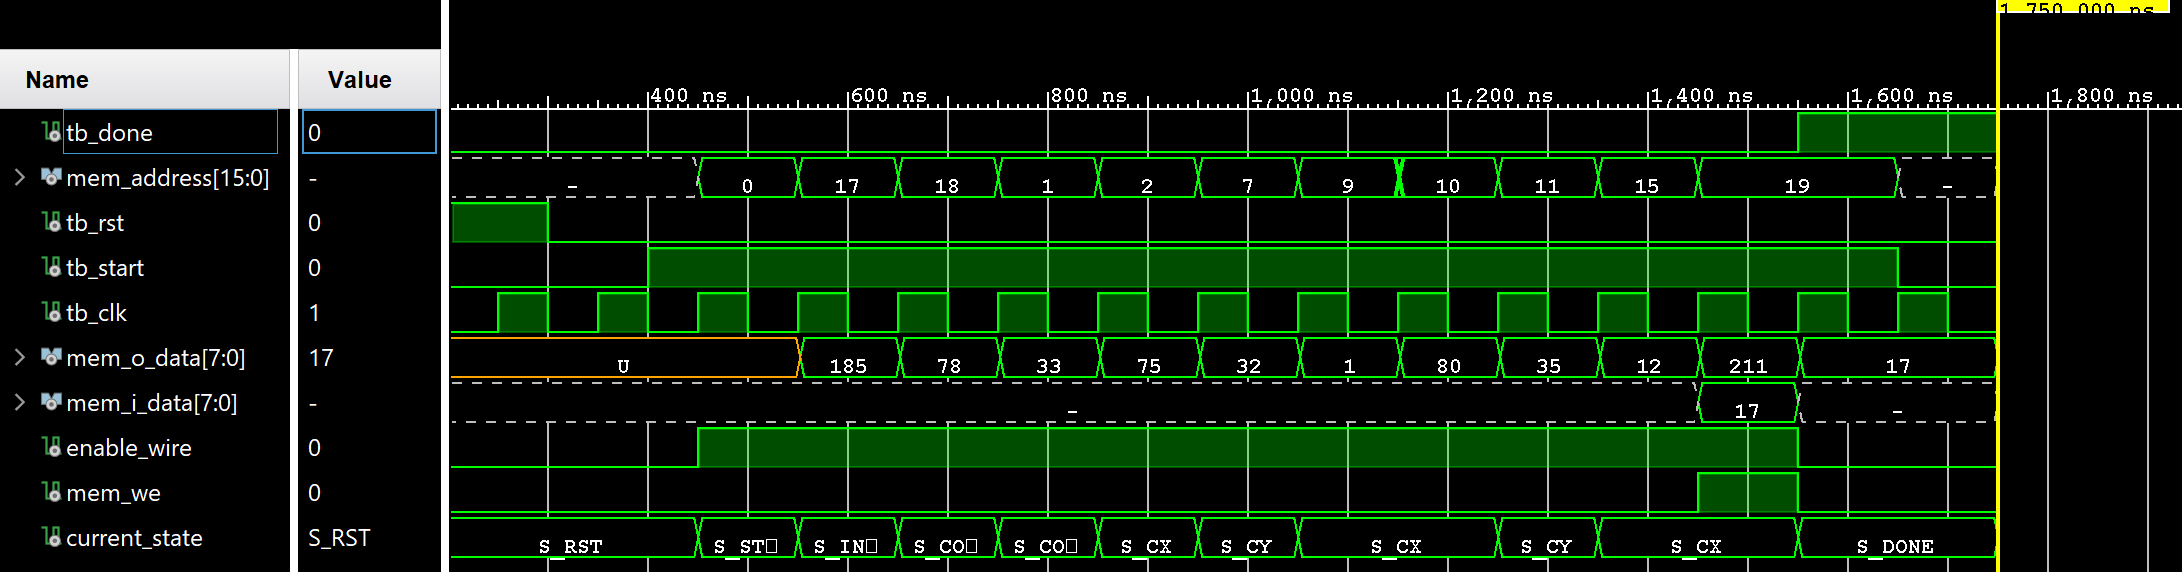
\includegraphics[width=1.0\textwidth]{images/test-bench-0.png}
    \label{fig:test-bench-0}
\end{figure}
Come si può vedere in figura \ref{fig:test-bench-0}, il componente impiega soltanto 11 cicli di clock dalla ricezione del segnale di start fino alla segnalazione di fine con \verb^o_done^.\\
Vediamo cosa succede in questi 11 cicli di clock con cui il componente arriva al risultato finale:
\renewcommand{\labelenumi}{\Roman{enumi}}
\begin{enumerate}
    \item Alla ricezione del segnale di start la FSM del componente passa allo stato \verb^S_START^, qui manda come indirizzo di lettura l'indirizzo 0.
    \item La FSM passa allo stato \verb^S_INPUT_MASK^. Il componente riceve il contenuto della cella di memoria 0: 185. Questa è la maschera d'ingresso che verrà salvata nel relativo registro. Infine manda come indirizzo di lettura l'indirizzo 17.
    \item La FSM passa allo stato \verb^S_COORD_X^. Il componente riceve il contenuto della cella di memoria 17: 78. Questa è la X del punto da valutare che verrà salvata nel relativo registro. Infine manda come indirizzo di lettura l'indirizzo 18.
    \item La FSM passa allo stato \verb^S_COORD_Y^. Il componente riceve il contenuto della cella di memoria 18: 33. Questa è la Y del punto da valutare che verrà salvata nel relativo registro. Infine manda come indirizzo di lettura l'indirizzo 1.
    \item La FSM passa allo stato \verb^S_CX^. Il componente riceve il contenuto della cella di memoria 1: 75. Questa è la X del primo centroide che verrà salvata nel relativo registro. Infine manda come indirizzo di lettura l'indirizzo 2.
    \item La FSM passa allo stato \verb^S_CY^. Il componente riceve il contenuto della cella di memoria 2: 32. Questa è la Y del primo centroide con cui calcola la distanza minima col punto da valutare. Infine manda come indirizzo di lettura l'indirizzo 7, \textbf{vengono quindi saltati i centroidi 2 e 3 siccome non sono da considerare per la maschera}.
    \item La FSM passa allo stato \verb^S_CX^. Il componente riceve il contenuto della cella di memoria 7: 1. \textbf{La distanza sulle ascisse tra questo centroide e il punto da valutare è maggiore della distanza minima. Perciò si passa al centroide successivo}. Manda quindi come indirizzo di lettura l'indirizzo 9.
    \item La FSM rimane nello stato \verb^S_CX^. Il componente riceve il contenuto della cella di memoria 9: 80. Questa è la X del quinto centroide che verrà salvata nel relativo registro. Infine manda come indirizzo di lettura l'indirizzo 10.
    \item La FSM passa allo stato \verb^S_CY^. Il componente riceve il contenuto della cella di memoria 10: 35. Questa è la Y del quinto centroide con cui calcola la distanza dal punto da valutare. Si trova che questa distanza è equivalente a quella minima, viene perciò attivato il quinto bit nella maschera di uscita temporanea. Infine manda come indirizzo di lettura l'indirizzo 11.
    \item La FSM passa allo stato \verb^S_CX^. Il componente riceve il contenuto della cella di memoria 11: 12. \textbf{La distanza sulle ascisse tra questo centroide e il punto da valutare è maggiore della distanza minima. Perciò si passa al centroide successivo}. Manda quindi come indirizzo di lettura l'indirizzo 15, \textbf{viene saltato il centroide 6 disattivato nella maschera}.
    \item La FSM rimane nello stato \verb^S_CX^. Il componente riceve il contenuto della cella di memoria 15: 211. \textbf{Anche qui la distanza sulle ascisse è maggiore della distanza minima}. Abbiamo perciò raggiunto il risultato finale: 0001'0001 (17). Esso viene mandato in scrittura alla RAM nella cella con indirizzo 19.
\end{enumerate}

\subsubsection{Post-Synthesis Timing Simulation}
Vediamo per questo test bench il comportamento del componente una volta sintetizzato.
\begin{figure}[H]
    \centering
    \caption{Test bench 0, waveform dei segnali in Post-Synthesis Timing Simulation}
    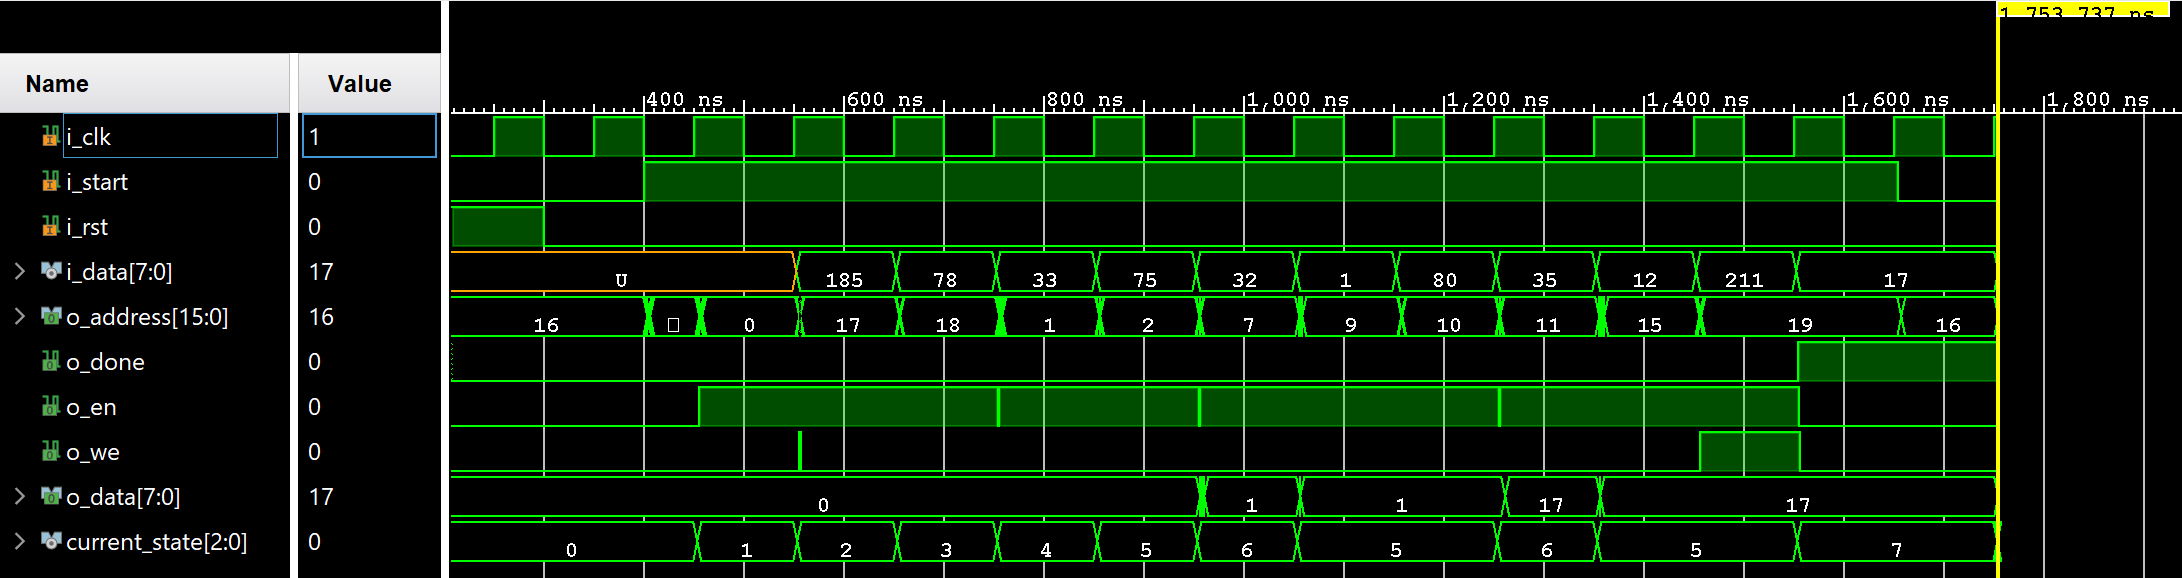
\includegraphics[width=1.0\textwidth]{images/test-bench-0-timing.png}
    \label{fig:test-bench-0-timing}
\end{figure}
\noindent I "don't care" spariscono e sono rimpiazzati da valori reali, questi valori sono ininfluenti e sono dati dalle ottimizzazioni fatte dal tool di sintesi. Inoltre sono comparse alcune alee statiche: di tipo 0 sul segnale \verb^o_we^ e di tipo 1 sul segnale \verb^o_en^. Queste alee sono ininfluenti per il risultato in quanto questi segnali sono usati in modo sincrono: conta soltanto il loro valore nell'intorno del fronte di salita del clock.

\subsection{Test Bench 1 (un solo bit attivato nella maschera d'ingresso)}
Con questo test bench si è voluto testare l'ottimizzazione n.2 della sezione \ref{subsection-ob-vel} a pagina \pageref{subsection-ob-vel}. Si è testato in realtà tutti i 9 casi possibili (zero bit attivati, un bit attivato in 8 possibili posizioni) ma vediamo soltanto uno di questi casi in quanto poi gli altri sono equivalenti.

\subsubsection{Dati del test bench}
\begin{table}[H]
    \begin{tabu*} to 0.8\textwidth { X[1.7l] X[1.1c] X[0.7c] X[1.1c]}
        \textbf{Contenuto} & \textbf{Valore} & \textbf{Indirizzo} & \textbf{Da considerare} \\
        Maschera d'ingresso & 1000'0000 (128) & 0 & - \\
        ... & ... & ... & \xmark \\
        X centroide 8 & 25 & 1 & \cmark \\
        Y centroide 8 & 23 & 2 & \cmark \\
        X del punto da valutare & 86 & 17 & - \\
        Y del punto da valutare & 129 & 18 & - \\
    \end{tabu*}
\end{table}

\subsubsection{Elaborazione}
\begin{figure}[H]
    \centering
    \caption{Test bench 1, waveform dei segnali in Behavioral Simulation}
    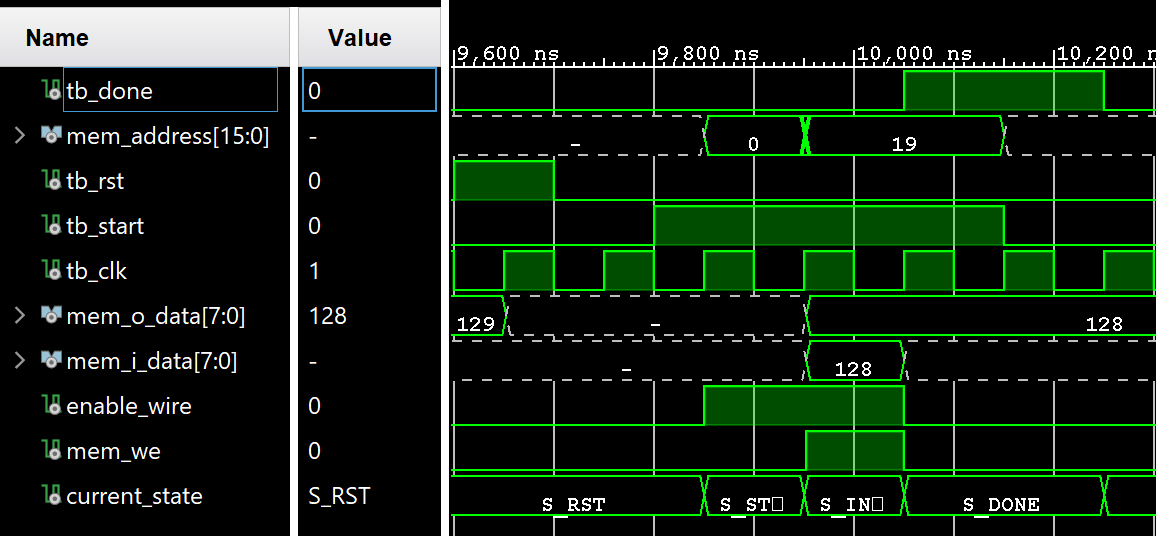
\includegraphics[width=0.6\textwidth]{images/test-bench-1.png}
    \label{fig:test-bench-1}
\end{figure}
Come si può vedere in figura \ref{fig:test-bench-1}, il componente impiega soltanto 2 cicli di clock dalla ricezione del segnale di start fino alla segnalazione di fine con \verb^o_done^.\\
Vediamo cosa succede in questi 2 cicli di clock con cui il componente arriva al risultato finale:
\renewcommand{\labelenumi}{\Roman{enumi}}
\begin{enumerate}
    \item Alla ricezione del segnale di start la FSM del componente passa allo stato \verb^S_START^ qui manda come indirizzo di lettura l'indirizzo 0.
    \item La FSM passa allo stato \verb^S_INPUT_MASK^. Il componente riceve il contenuto della cella di memoria 0: 128. A questo punto la funzionalità di assegnamento del segnale \verb^is_immediate^ riconosce che la maschera d'ingresso è una potenza di due. Ciò viene riconosciuto se \(128\&(128-1)\) dà come risultato 0, ed effettivamente si trova che 1000'0000 \& 0111'1111 = 0000'0000. Si è quindi raggiunto il risultato finale che non è altro che la maschera d'ingresso stessa: 128.  Esso viene mandato in scrittura alla RAM nella cella con indirizzo 19.
\end{enumerate}

\subsection{Altri test bench}
Sono stati creati altri test bench per testare alcuni casi limite o per controllare la robustezza del componente. Non li vediamo in dettaglio siccome alla fine seguono tutti lo stesso principio di esecuzione.
\begin{itemize}
    \item Test bench in cui la distanza del punto da valutare coi centroidi è molto alta e tale per cui si devono usare 8 + 1 bit. Si è usato quindi dati in cui il punto da valutare ha ascissa e ordinate dal valore molto basso mentre per i centroidi si è usato sia per la X che la Y valori maggiori di 200.
    \item Test bench in cui alcuni centroidi sono a distanza 0 con il punto da valutare.
    \item Test bench in cui tutti i centroidi sono da considerare e hanno la stessa distanza col punto da valutare (maschera di uscita: 1111'1111).
    \item Test bench in cui si controlla il corretto funzionamento del componente a seguito di elaborazioni successive senza segnali di reset.
    \item Test bench in cui si controlla il corretto funzionamento del componente quando, durante una elaborazione, viene mandato un segnale di reset.
    \item Infine sono stati creati una decina di altri test che non vanno a verificare casi particolari ma semplicemente casi normali con dati diversi. Questi test sono stati progettati in modo che ogni bit nella maschera di uscita venga testato almeno una volta.
\end{itemize}
\begin{figure}[H]
    \centering
    \caption{Esempio di test bench effettuato con elaborazioni successive}
    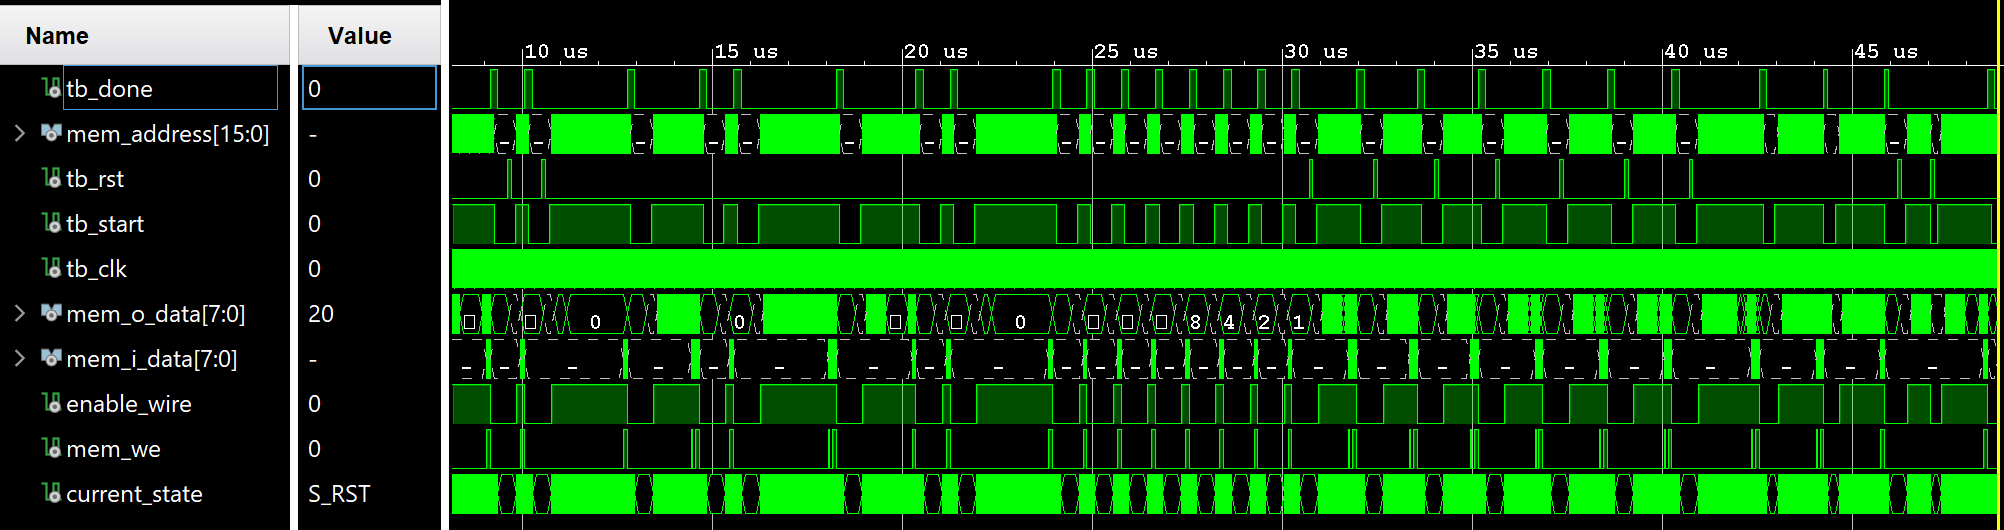
\includegraphics[width=0.95\textwidth]{images/altri-test-bench.png}
    \label{fig:altri-test-bench}
\end{figure}

\vspace{4mm}
\titlerule[0.4pt]


%%%%%%%%%%%%%%%%%%%%%%%%%%%%%%%%%%%%%%%%%%%
%%%%%%%%%%%%%%% CONCLUSIONE %%%%%%%%%%%%%%%
%%%%%%%%%%%%%%%%%%%%%%%%%%%%%%%%%%%%%%%%%%%
\section{Conclusione}
Riassumendo si è creato un design con queste caratteristiche:
\begin{itemize}
    \item Funzionante in pre e post-sintesi.
    \item Ottimizzato in modo che durante l'elaborazione venga sfruttata al massimo la RAM: a ogni ciclo di clock una lettura o una scrittura.
    \item Ottimizzato in modo che ogni lettura della RAM venga eseguita solo se strettamente necessaria (non viene letto ciò che non serve).
    \item Configurabile con le costanti \verb^MEM_BITS^ e \verb^CELL_BITS^ per adattarsi a differenti tipi di RAM, e con il generic \verb^START_ADDRESS^ per eseguire l'elaborazione all'indirizzo desiderato.
    \item Frequenza massima di clock impostabile a 85.6Mhz.
    \item Utilizzo di LUT pari al 0.15\%.
    \item Utilizzo di FF pari al 0.02\%
\end{itemize}

\end{document}
